\chapter{Methodology}\label{chapter:methods}

This chapter describes implementation of the mobile Augmented Reality (AR) pipeline of avatars rendering, and experiments on increasing the DNN's \cite{dnn:stylepeople21} images quality for AR scenario. Section \ref{methods:dev-setup} lists target hardware and software, including the used libraries, tools, and configuration of the baseline model. Section \ref{methods:app} describes the mobile pipeline and algorithmic tricks used to achieve real-time performance. Section \ref{methods:zooms} presents motivation and implementation details for experiments with the DNN's training procedure.

\section{Experimental setup}\label{methods:dev-setup}

The baseline DNN \cite{dnn:stylepeople21} model can be trained on a monocular video sequence of frames with a single person shown from multiple sides. There are several pre-made training video sequences with different people at our disposal. They were captured for approximately 1 minute on a stationary monocular smartphone camera, in resolution $1920 \times 1080$ pixels. Only each 8th frame from the video was retained to get a representative set of distinct body poses. Then, for each frame a segmentation mask was predicted using an external pretrained segmentation model Graphonomy \cite{dnn:graphonomy19}, to replace color of background objects with 0 values. Next, SMPL-X \cite{dnn:smplx19} body model was fit to all the frames, i.e. predicting pose vector $\theta$, facial expression vector $\psi$, and body shape vector $\beta$. The latter is purposely predicted to be the same across all the frames, in order to bias the DNN to synthesize images for this body shape only, which will be exploited in real-time inference on mobile in Section \ref{methods:app}. Using body model fits, a posed body mesh for each frame can be obtained as was described in Section \ref{lit:nrender}. 

Sometimes, 3D model fits may be misaligned with complicated ground truth 2D frames, e.g. due to complex twists and bending of joints, occluded body parts. To reduce the effect of training the DNN on outlying unstable inputs, many of the falsely fit ground truth images were manually filtered out from the training set. It was observed, that the quality of body model fits is critical for the avatars final quality. Hence, for the scope of this thesis, we decided to take a single training sequence, that has the best body model fits we could obtain. The training pipeline adjustments discussed in Section \ref{methods:zooms} will be primarily applied to this training sequence. This also allows the fair quantitative and qualitative comparison. For simplicity, when we further mention \textit{the training sequence}, we mean this single training sequence. A few promising experiments will be repeated with a few other sequences to verify stability of results (for example, see Figure \ref{fig:exp:instancenorm-other-seq}). 

After filtering out the bad frames, the training sequence contains 410 samples. Out of them we holdout 13 frames as a validation set. It includes 11 consecutive frames from a frontal view, in poses that do not resemble any other training data; and also 2 frames with side and back view. As for a test set, we made a sequence of continuous difficult poses and camera angles. It includes an animation with extensive hands gesturing, a view on the avatar from top, bottom, far away, and close-up to the face. The test sequence is completely unrelated to the training data and was designed by us to verify that the DNN is capable of rendering frames that may be encountered by a user in an AR session. The possible visual artifacts may include flickering between two similar frames, clothes shaking, color shifts, blurriness, etc. See Appendix Section \ref{appb:exps}, featuring a few training and test images that we use. Lacking an absolute metric of visual quality, in this research we mainly rely on manual inspection and comparison of the test video sequences. 

In the next paragraphs we will elaborate more on the specific configuration of the baseline DNN architecture, that was first mentioned in Section \ref{lit:nrender}. By default, we stick to $512\times512$ pixels resolution of synthesized images. Both the ResNet18 encoder and decoder of the neural renderer consist of 5 levels of 2-layer CNNs with stride 2 and kernel sizes either $3\times3$ or $5\times5$. The U-Net yields a tensor with 64 channels and the original spatial resolution. Two independent CNNs with 2 layers each (also called heads) then map it into a 3-channel RGB image, and a 1-channel segmentation mask, that are concatenated into the final RGBA avatar image.

%$C \times 512 \times 512$ ($C$ is number of input channels and $512 \times 512$ is spatial resolution) is enlarged to $64$ channels, and processed by 5 sequential levels, each consisting of 2 convolutional layers. Through the levels, the size of activations follows the sequence: $64 \times 256 \times 256 \rightarrow 128 \times 128 \times128 \rightarrow 256\times64\times64 \rightarrow 512\times32\times32$. The resulting activation is then passed through the decoder part, where it gets upsampled to twice as bigger spatial resolution, then it is concatenated with the second to last encoder level's activations. The decoder level ends with a convolutional layer. The same procedure is repeated for the remaining decoder levels, concatenating with features of the corresponding encoder levels. Finally, on tensor size $64\times512\times$, the channels depth is shrunk to 16, and .

The neural texture is a tensor of 16 channels and resolution $512\times512$ by default (although may be arbitrary). For the SMPL-X body model mesh, there is a known mapping from 3D mesh vertices to the same 2D texture image coordinates (as on Figure \ref{intro:fig:mesh-texture}), regardless of body shape (tall, short, slim or obese). In addition to the original resolution, extra texture scales of size $16\times 2^k \times 2^k, \forall k \in \{3,..,8\}$ are created and jointly optimized. This set of scales is referred to as a multi-scale neural texture. Before rasterizing the body mesh, all the scales are upsampled to $512$ resolution and averaged into a single texture. The multi-scale texture allows to share information among adjacent vertices and proven to reduce flickering of the output avatar images. Also, the baseline neural texture uses a special initialization. It is computed as spectral coordinates of vertices on the graph, that is made out of the body mesh. In short, the graph's Laplacian matrix is calculated, and Eigenvectors of it are called spectral coordinates \cite{aux:spectral10}. A few first dimensions of these vectors are used to initialize the neural texture. The purpose of such initialization is in separation between different parts of the body (see Figure \ref{fig:spectral_ntex}), e.g. there are channels that assign opposite values to left/right limbs, or lower/upper body, or adjacent fingers and so on. Such initialization helps to guide the neural renderer to uniquely distinguish the body parts, improving convergence speed.

During training, the synthesized image and its segmentation mask are supervised with a weighted sum of training losses. By default Dice, L1, LPIPS (VGG \cite{dnn:vgg14} based), Adversarial and Feature Matching losses are used, with weights 25, 25, 20, 1, 1 respectively. The adversarial loss is a Binary Cross Entropy (BCE) loss of predictions made by an ensemble of $N=3$ discriminator networks. Each discriminator is a CNN that gradually decreases the spatial resolution and increases the number of channels, until finally a Sigmoid function returns a probability in range $[0;1]$ of the image being real. The discriminators are supervised to improve their accuracy on both synthesized and real images, while the neural renderer is supervised to decrease discriminators' accuracy for the synthesized ones. See Formula \ref{methods:eq:bce} for BCE, when computing it for a real image $x$, then $y$ is set 1 for discriminators; if $x$ is a generated image, then $y$ is 0 for discriminators, but 1 for the neural renderer.
\begin{equation}
	BCE = - \dfrac{1}{N} \sum_{i=0}^N y \cdot \log_{2}(D_i(x)) + (1-y) \cdot \log_{2}(1 - D_i(x)) 
	\label{methods:eq:bce}
\end{equation}

Adam \cite{dnn:adam14} optimizer is utilized for training of the neural renderer, neural texture and discriminators. They are optimized with learning rate (LR) of $10^{-3}$, $10^{-3}$ and $10^{-5}$ respectively. By default, the Adam's first and second momentum values are 0.9 and 0.999 respectively, without weight decay (also known as L2 penalty on norm of the optimized parameters).

In the baseline training process, a batch of random training samples is selected. Using body model's mesh, a bounding box is found that tightly encloses the person's extents on the ground truth image. The image is cropped by this bounding box using bilinear interpolation to get a $512 \times 512$ image with the person's body in the image center. With the same resolution and alignment, the body mesh is rasterized. Then, both the ground truth and rasterization are processed with image-space augmentations (see Figure \ref{fig:image-space-aug-kornia}), that perform random affine rotation, scale and translation of the image to improve generalization of the neural renderer to different camera views on the same avatar. Then the neural renderer is infered with input rasterization, and loss is computed between real and synthesized images. The gradient is computed and applied to all the learned parameters (the neural texture, neural renderer and discriminators) on every single batch. We train the pipeline on desktop hardware -- one GPU NVIDIA Tesla P40. It takes about 16 hours to complete a single experiment of 500 epochs on about 500 frames of ground truth images, with batch size 8 and resolution $512\times512$ pixels. All training computations are carried out in full-float FP32 numbers format. As validation metrics, we compute LPIPS (AlexNet \cite{dnn:alexnet12} based), SSIM, MS-SSIM, and PSNR, as well as tracking values of L1, Adversarial and Dice losses on the validation set.

The experimentation on deep neural networks is carried out in Python programming language and PyTorch framework for the DNNs training. We use many Python libraries for data processing and visualization: NumPy, Matplotlib, OpenCV, Pillow, Open3D. In order to optimize parameters of the neural texture, it needs to be rasterized with the body mesh using differentiable rendering algorithm, we use Nvdiffrast library for that \cite{aux:nvdiffrast20}. The image-space augmentations need to be differentiable for the same reason, for which we utilize Kornia library \cite{aux:kornia20}.

The primary mobile hardware that we target with our mobile application is SoC Qualcomm Snapdragon 888, which is one of the latest high-end platforms that features a fast and power efficient DSP computing unit for AI, and high throughput for processing mobile camera data in real-time. Although the preceding versions of the platform also contain the DSP, they are too slow to infer the baseline DNN in real-time. Qualcomm Snapdragon 835 is the oldest platform that we succeeded to launch the mobile application on, although with unacceptable performance.

We develop the mobile application in Java and Kotlin programming languages. The development environment consist of the Java Software Development Kit (SDK) and Android SDK. We perform installation of the compiled code on a mobile device via Android Debug Bridge (ADB) software utility. In order to launch the PyTorch DNN on mobile, first of all we use Snapdragon Neural Processing Engine SDK (SNPE, \cite{aux:snpe}). It includes Android runtime libraries, as well as desktop software tools for conversion of DNN architectures into binary files, that can be loaded onto mobile devices and executed. Among the tools there is a utility for post-training quantization of a neural architecture. We supply it with 5-10 input frames from the test sequence. The neural renderer network is inferred with those frames, and the range of quantization is computed for each intermediate tensor. Then all the weights are quantized as was described in Section \ref{lit:dnn-speedup}. The direct conversion of PyTorch DNN models into SNPE format is not supported, however there is an Open Neural Network Exchange format (ONNX, \cite{aux:onnx}), which supports conversion from PyTorch to ONNX (provided by PyTorch), and from ONNX to SNPE (provided by SNPE SDK). The final file with the quantized DNN is passed along with the quantization constants to the mobile application to accordingly generate quantized input frames.

On the mobile application's side, we use SNPE Android Runtime library to load the model's file and to specify performance profiles. Those control how much of computing power should be devoted by the device. We use "Sustained High Performance" profile, since we intend to continuously infer the DNN over a long period of time with low latency. On the other hand, there is the absolute highest performance profile, that would lead to the best performance over a short period of time, that would drastically decrease upon reaching the overheating limit. Prior to inference, SNPE should be given with pointers to memory locations, where to read the input data, and where to write the output data. We accordingly preallocate buffers on CPU and GPU, and use them for the whole run of the mobile application to minimize costs of memory allocation on each frame.

For the DNN inference, we need to generate an input frame (see Figure \ref{lit:fig:stylepeople}), that would show the body mesh oriented as an object of Augmented Reality. Hence, the orientation should correspond to the mobile device's camera. This requires continuous tracking of camera position in the real world, as well as positions of the surrounding environment. We use ARCore SDK \cite{aux:arcore22} that provides it with little programming required. It uses inertial measurement units, camera images and depth sensor of the device to keep track of distinct points in the camera view. This allows to estimate proximity of the real world objects, and to reconstruct vertical and horizontal flat surfaces, such as floors, desks, walls. The location and bounds of these surfaces can be queried from the ARCore. It also allows to place and track anchor points on the detected surfaces. The tracking information can be retrieved from ARCore in a form of transformation matrices of the anchors and camera (extrinsics, as in Formula \ref{lit:eq:extrinsic}). The projection matrix of the camera (intrinsics, as in Formula \ref{lit:eq:intrinsic}) can also be retrieved, allowing to render images that span the whole screen of the device. 

The generation of input frames is in essence a classic rasterization of a triangular mesh onto an image using a 2D texture. This process can be delegated to the high-performance graphics library, which is called Open Graphics Library (OpenGL, \cite{aux:opengl22}). It provides low-level control of a GPU device, to layout and are pre-process the data of meshes and textures. Then, using GPU programs written in OpenGL Shading Language (GLSL, \cite{aux:glsl21}), also referred to as shader programs, we can make linear algebra computations on individual vertices of the mesh (vertex shader), or individual pixels on the rendered image (fragment shader). Since all those primitives can be processed independently, this computation is automatically parallelized on GPU by OpenGL, thus achieving very high performance of rasterization. We also use it to render camera frames on the screen. On top of them we render the avatar images, resulted from the DNN's inference (see Figure \ref{fig:mobile_example}). In fact, we use a subset of the library, called OpenGL for Embedded Systems (OpenGL ES) version 3.2, that consists of core functionality for rasterization, lacking many high-end graphical extensions.

The application is compiled with all performance optimizations enabled. The frame time of the mobile AR experience is measured directly in the application. We report timings of processing steps of the current frame via logging, namely: time of SMPL-X body mesh inference from a pose vector, time of rendering the DNN's input frame on GPU, time of delay between obtaining this data and receiving it on the DNN's side, time of DNN's inference, time of rendering the inferred outputs on the screen. However we notice, that by far the highest processing time is taken by the DNN inference step. To measure its timings more accurately, we created a separate mode for the application, which we call "benchmarking". In this mode, the only thing that is being calculated is continuous inference of the DNN for a few minutes with a constant random tensor of data. Thus, the computing device will be maximally utilized with the DNN inference only. We consider it an upper bound of the power consumption and heat generation. The benchmarking reports increase in temperature and average timing of DNN inference. We additionally use Qualcomm Snapdragon Profiler software. It allows to capture hardware metrics of a running mobile application. From that, we visualize occupation of computing devices over time, and reason about potential bottlenecks.

\section{Mobile application development}
\label{methods:app}

The Android mobile application was developed from scratch specifically for this Master thesis. A considerable amount of technical work was spent on implementing the general functionality of the application. This includes:
\begin{itemize}
	\item system events handling, such as opening, closing, resuming from the operating system;
	\item requesting of system permissions on camera and hard drive storage;
	\item adding binary files into an installation package, including runtime libraries, files of quantized DNN models, neural textures, configuration files, assets for inference of SMPL-X, etc;
	\item setup of logging;
	\item reacting to user interaction, such as finger taps, swipes, pinch movements;
	\item populating the user interface with options to select a  particular DNN for inference, options of DNN input generation, predefined animations, features of rasterization, etc. 
\end{itemize}

We publish only a part of the code base which is the most relevant to synthesis of avatar images on mobile, that is described in the following paragraphs (See Appendix \ref{appendix-code}).

We initialize OpenGL library, by creating a \verb|Surface| object from the Android SDK, that spans the whole screen of the device, and specifying it as a context of OpenGL to render to. This creates a separate execution thread on CPU. Only on this thread the commands of OpenGL (and thus GPU processing) can be executed. We configure the context to use 8 bits for all color channels of the screen and 32 bits for values in the Z-buffer. In OpenGL all the data is allocated on GPU as contiguous arrays, and the library has to be programmed how to interpret these arrays. The triangular meshes can be defined by a flat array of vertex attributes, where consecutive elements contain attributes of a single vertex. The most basic scenario is to pass an array of $\langle x, y, z, u, v\rangle$ with $xyz$ being a 3D vertex position in a local coordinate space of the modeled object, and $uv$ being texture coordinates of the vertex. Also, a connectivity array has to be provided in a form of indices in the array of vertex attributes. Three consecutive indices form a single triangle. We use back-face culling throughout the rendering, meaning that OpenGL will not render triangles facing away from the camera, slightly improving performance by culling some triangles out of processing. To define which triangles are facing away, we specify to interpret vertex indices as clockwise triangles, meaning that a triangle of indices $\langle a, b, c\rangle$ will face towards the camera if and only if after projecting on the screen the vertices appear in a clockwise order. Overall, we use three separate triangular meshes, one for SMPL-X human body mesh (described further), and two "meshes" which are essentially rectangles. The first one is rasterized, spanning the whole screen, and taking color values from a texture that contains a current camera frame. The other one is similarly rasterized, but at a location of the avatar, taking values from a texture loaded with output of the inferred DNN (See a debugging illustration from the mobile application on Figure \ref{fig:far_dynamic_crop_debug}).

OpenGL doesn't support storage or rasterization of images with more than 4 channels (Red-Green-Blue-Alpha only). We need to load the neural texture of $C$ channels on GPU. If it is a multi-scale texture, we convert it into a single scale, by averaging all the scales into the $C \times 512 \times 512$ texture scale. Then we split it by 4 channels and load these parts as separate arrays on GPU. However querying of multiple textures requires extra processing time in OpenGL fragment shader programs. We thus create an OpenGL's Array Texture data structure, that improves querying of multiple textures with the same texture coordinates, which is exactly how we use these texture parts. We use FP16 format for storage, to a reduce memory footprint of the texture compared to FP32. This also should result in better utilization of texture memory caches inside GPU. OpenGL allows to apply an additional filtering algorithm on textures, to generate multiple scales of the texture, which are called MIP-maps (see Figure \ref{fig:mipmap}). Those can be used to render triangles that span very little area on the screen. The filtering prevents blurriness and aliasing artifacts from appearing due to bilinear sampling. Furthermore, anisotropic filtering can be applied to also generate stratched variants of scales. It improves quality of rendering triangles that face at steep angles to the camera (see Figures \ref{fig:anisotropic} and \ref{fig:anisotropic_result}). Both methods require extra texture memory: about x2 for MIP mapping, and up to x16 for anisotropic filtering, and slightly more processing time. However, given the small resolution of our textures and relatively low triangle count in the body model, we found the performance difference to be negligible. We would like to clarify the confusing terminology. The multi-scale texture exists only in the DNN pipeline in Python, the scales of it are upsampled and averaged before rasterization. The texture  MIP maps in the mobile application always remain at lower resolutions, and a GPU driver heuristically selects an appropriate MIP-map to render a certain triangle.

Next we initialize a tracking session of ARCore library. It starts intercepting and processing the camera frames on GPU, allowing to refer to the camera data as an OpenGL texture. By default, ARCore processes a new camera frame and awaits for the next to arrive. The application is then capped to the camera's update rate -- 30 frames-per-second (FPS) for our devices. We configure ARCore to never wait and process the current camera frame, regardless if it was already processed. This allowed us to cap the application to the Android's internal limit of 60 FPS.

As was mentioned in Section \ref{methods:dev-setup}, we initialize SNPE DNN models with "Sustained High Performance" profile, and the computing unit specified by the user (supporting either GPU or DSP). GPU offers better support of neural layers used in DNN models, since it can perform computations in FP32 or FP16 format, analogously to a desktop GPU. But running a DNN on it would also mean that input rasterization and DNN inference would have to be done one after another, possibly bottlenecking the performance. On the other hand, DSP offers much higher performance than GPU, and inference can take place independently and in parallel with our input generation on GPU. However, the usability of DSP is very limited, e.g. much fewer neural layers support quantized computations; also loading of the DNN models requires long initialization, up to several minutes. Besides, Qualcomm Snapdragon's DSP contains a hardware security policy, that only allows to run on consumer devices the programs, that were certified by the hardware vendor. We ignore this issue for our project, by having test engineering samples of smartphones that suppress this security check. If SNPE fails to load a model on DSP, it may fallback to using GPU, or even CPU execution, obviously being extremely slow for inference.

Finally, before inference, we can pre-compute parts of the SMPL-X \cite{dnn:smplx19} body mesh. Since it's only done once, we do this computation on CPU. We load 3D positions of $N$ vertices in the template mesh with a rest body pose. Then, following the algorithm (see at the end of Section \ref{lit:nrender}), for mobile inference we'll use the same body shape vector $\beta$ that was used during DNN training. From $\beta$ we can compute a linear component $B_S(\beta; \mathcal{S})$ as in Formula \ref{lit:eq:smplx-components}, that offsets the template vertex positions to represent the specific body constitution of the avatar. We compute it is as a multiplication of a tensor with shape $N \times 3 \times \lvert\beta\rvert$ (provided by SMPL-X) and the $\beta$ vector (from the dataset), yielding the offsets $N \times 3$ that we add to the template vertex positions. We similarly compute the $B_E(\psi; \mathcal{E})$ linear component, that offsets vertices of the face. Although the face shape can slightly change between different facial expressions, we only compute the linear component once before inference, for simplicity. Lastly, SMPL-X includes a pretrained linear regressor of joints 3D positions, from all the mesh vertices. We also pre-compute this regression, which comes down to computing multiplication of the regressor's matrix $55 \times N$ and the mesh vertex positions $N \times 3$, yielding the 3D positions of 55 body joints. 

During inference, the pose-dependent linear component has to be computed and added for each frame in order to get a posed body mesh. As was already described, it involves finding a weighted sum of 55 affine transformation matrices of size $4 \times 4$, with a separate set of weights for each vertex. The weights define how strong the rotation of a particular joint affects offset of the vertex (for example, see Figure \ref{fig:smplx-vert2joint}, how some vertices are dominantly affected by a particular nearby joint). Having approximately 10 000 vertices in the mesh, we need to multiply and add a total of $55 \cdot 10 000 \cdot 4 \cdot 4 = 8 800 000$ floating-point values on every frame. This computation would be time consuming on CPU, but since it can be trivially parallelized, we instead pre-allocate the array of weights in OpenGL (on GPU), and compute the weighted sums in the vertex shader program. We further noticed, that among 55 weights per vertex at least 43 are zeros. Thus we can improve the performance, by sorting the weights on CPU during the pre-processing step, and allocating on GPU only 12 most significant weights  and their joint indices $i \in \{1,...,55\}$. Overall, we load on GPU the pre-computed shaped vertex positions $\langle x, y, z \rangle$, texture coordinates $\langle u, v \rangle$, joints weights $w_k$ and joints indices $i_k$ as an array of vertex attributes on GPU. We use an interleaved layout, where $\langle x, y, z, u, v, w_1, .., w_{12}, i_1, .., i_{12}\rangle$ of a single vertex are located contiguously in the GPU array, improving memory cache efficiency of posing a single vertex. 

Next, we will describe the interactive stage of the application, which is an infinite loop of computing and rendering the AR experience. Each frame starts by inferring the pose-dependent linear component $B_P(\theta; \mathcal{P})$ of SMPL-X. It is computed from a pose vector $\theta$, containing $3 \cdot 55$ values with axis-aligned rotation vectors for all the joints. A single rotation vector $\bmr{r} = \langle r_x, r_y, r_z \rangle$ needs to be converted into a $3\times3$ rotation transformation matrix $\bmr{R}$, using Rodrigues \cite{aux:rodrigues11} formula (we use $\bmr{I}$ for an identity matrix):
\begin{equation}
	\bmr{R} = \bmr{I}_{3\times3} + \text{sin}(\|\bmr{r}\|)\cdot \bmr{A} + (1-\text{cos}(\|\bmr{r}\|))\cdot \bmr{A}^2,
	\quad \text{where} \quad
	\bmr{A} = \dfrac{1}{\|\bmr{r}\|}
	\begin{bmatrix} 
		0 & -r_z & r_y \\
		r_z & 0 & -r_x \\
		-r_y & r_x & 0
	\end{bmatrix}
	\label{methods:eq:rodrigues}
\end{equation}

The joints apply their rotations and translations recursively, e.g. a position of a finger can be found from sequentially applying transforms of the arm, forearm, palm, and every knuckle. We could compute each joint's final transformation independently, by multiplying all chains of the matrices. However, we can exploit the fact, that the joints form a tree structure, i.e. every joint depends on only one parent joint without loops. Thus, we use a topologically ordered array of 55 joints, meaning that no joint in the array precedes its parent joint. This allows faster CPU computation for $4\times4$ transformation matrices of joints, because by the time we process a joint $i$, all its dependent transformations are already computed in a form of a single matrix of its direct parent. We take 3D locations of joints $\bmr{t}$ (regressed during the initialization stage), and get relative joint translations $\Delta\bmr{t}$ by subtracting joints positions from their parents'. The final recursive transform \bmr{H} for a joint $i$ is found as:
\begin{equation}
	\bmr{H}_i = 
	\bmr{H}_p
	\cdot
	\begin{bmatrix} 
		\bmr{R}^i_{3 \times 3} & \Delta\bmr{t}^i_{3 \times 1} \\
		\bmr{0}_{1 \times 3} & 1 \\
	\end{bmatrix}
	\cdot
	\begin{bmatrix} 
		\bmr{I}_{3\times3} & -\bmr{t}_i \\
		\bmr{0}_{1 \times 3} & 1 \\
	\end{bmatrix}
	\label{methods:eq:smplx-rodrigures-4by4}
\end{equation}
where $p$ is a parent index, the transformation matrix $\bmr{H}_p$ of which is already found by the time we compute $H_i$. The first matrix multiplication computes a relative recursive transform for the joint, and the second multiplication subtracts the true posed location of the joint. From the programming point of view, to save on computations, we implement the matrix multiplication operations not naively, but by expanding and merging the operations together, e.g. computing each element of $\bmr{R}$ matrices in place. We try to iterate the data in memory in a cache-friendly way, to write the data consecutively. We expect that it helps to retain exclusive usage of cache lines, without overhead of cache synchronization. For the full SMPL-X inference implementation, head to Listing \ref{appendix-code:smplx}.

Then, we extract tracking information from the ARCore session, namely camera intrinsic and extrinsic matrices, as well as transformation matrices of the tracked anchors. We pre-multiply the anchor's matrix by camera extrinsic matrix, and then by the intrinsic matrix, obtaining a single transformation from local body mesh coordinates to projected image coordinates. Unlike the classic representation of intrinsics, as in Formula \ref{lit:eq:intrinsic}, OpenGL uses an equivalent representation, but with another notation, called Native Device Coordinates. Formerly, the projection frustum was defined with a $3 \times 4$ matrix, parameterized with image width and height $W/H$, focal lengths $f_x/f_y$ from the pin-hole to the image, and image center offset $c_x/c_y$ in pixel coordinates. In OpenGL, the frustum is set by a $4 \times 4$ matrix via 6 distances that bound the frustum: top $t$, bottom $b$, left $l$ and right $r$ planes; a near plane $n$, analogous to focal distance; and a far plane $f$, which defines the maximum depth that is mapped by the virtual camera. The matrix has $4 \times 4$ size in order to additionally compute depth of each pixel, allowing to store it in a Z-buffer, and querying if some rasterized pixels are being occluded. We can represent the same projection with either notation:
\begin{equation}
	\bmr{K_{NDC}} \overset{\begin{subarray}{l}\text{previous} \\ \text{notation}\end{subarray}}{=} 
	\begin{bmatrix} 
		\tfrac{2f_x}{W} & 0                & \tfrac{W - 2c_x}{W}  & 0 \\ 
		0               & \tfrac{2f_x}{H}  & \tfrac{H - 2c_y}{H}  & 0 \\
		0               & 0                & -\tfrac{f + n}{f - n} & \tfrac{-2fn}{f - n} \\
		0               & 0                & -1                   & 0
	\end{bmatrix} \overset{\begin{subarray}{l}\text{OpenGL} \\ \text{notation}\end{subarray}}{=} 
	\begin{bmatrix} 
		\tfrac{2n}{r - l} & 0              & \tfrac{r + l}{r - l} & 0 \\
		0               & \tfrac{2n}{t - b}  & \tfrac{t + b}{t - b} & 0 \\
		0               & 0                & -\tfrac{f + n}{f - n} & \tfrac{-2fn}{f - n} \\
		0               & 0                & -1                   & 0
	\end{bmatrix}
	\label{methods:eq:ndc-projection}
\end{equation}

There are a few changes required for this projection matrix. Since we use it to rasterize an input frame to the DNN, we have to supply square images ($512 \times 512$ pixels resolution). However the default projection matrix has aspect ratio of the device's screen. The frustum can be squeezed, e.g. along vertical $y$ axis, by multiplying the second row of $\bmr{K_{NDC}}$ by the screen dimensions ratio $W / H$. Additionally OpenGL stores images from a bottom row to top, meaning that it appears vertically flipped when we use it outside OpenGL. To solve it, the element at second row and second column can be negated.

Now that we have posed joints, in order to pose all the mesh vertices we send the transformation matrices $\bmr{H}_i$, as well as the merged matrix of extrinsics and intrinsics on GPU, as uniform\footnote{The term \textit{uniform} is specific to OpenGL, it means that a single variable value is shared across all the primitives (vertices/pixels) processed by a shader.} variables of the vertex shader program (see Listing \ref{appendix-code:vertexshader}). Here, for each body mesh vertex we combine the most significant joints weights with corresponding matrices, taken by index offset specified in the vertex attributes. Notice, that when we compute \verb|uniqueVertexTransform| matrix, we don't add up the matrices plainly like $a + b + ... + g + h$, instead we use a scheme $((a + b) + (c + d)) + ((e + f) + (g + h))$. Due to the order of operations execution, the former variant requires to compute $a + b$, and only after that compute $(a+b) + c$ and further, even if hardware has multiple Multiply-Accumulate circuits (MAC) available. With the latter variant, we force computation of 4 inner sums independently, and then add them into the final matrix. This little reordering can optimize the performance, since its effect scales with the number of vertices. The vertex shader terminates by transforming the vertex with the affine transform, and projecting it into the screen coordinates. 

Then OpenGL automatically performs rasterization into an image. OpenGL interpolates vertex attributes and passes them into a fragment shader program, which is executed for all image pixels (see Listing \ref{appendix-code:fragmentshader}). We use interpolation of texture coordinates, to sample the neural texture in agreement with the texture unwrapping, and construct the pixels of the DNN's input tensor. SNPE processes the tensors in Batch-Height-Width-Channel layout (BHWC), i.e. all channel values of a single pixel are followed by channel values of the next pixel. On the bright sight, OpenGL uses exactly the same layout for rendered images. However once again, we stumbled upon a limitation of OpenGL that it cannot generate images of more than 4 channels, while we need $C$ channels. One solution is to render $\lceil \tfrac{C}{4} \rceil$ images of size $512 \times 512 \times 4$ using OpenGL on GPU, and then to permute the data in CPU memory to make a single tensor $512 \times 512 \times C$, and pass it to the DNN. However, it was proven to be extremely slow, even if this permutation is embedded into the DNN architecture, which may get some acceleration from the DSP device. Instead, recall that SNPE works with quantized input data, with INT8 per each channel value. We found a way to generate in OpenGL images with 4 bytes allocated per each image channel, thus having up to 16 bytes per pixel. Now, by passing quantization constants into the fragment shader, we can sample the floating point numbers from the texture, and using the quantizing transformation (see Formula \ref{lit:eq:float-to-quantized}) we obtain an INT8 value, which can be bit-shifted into an arbitrary byte of a particular channel. Thus, we can successfully pack input images with up to $C = 16$ channels using a single rasterization, without requiring \textit{any} additional processing on the DNN side - it can immediately start inferring from this data layout. The background pixels on the image that don't belong to the body mesh have to be handled carefully. By default OpenGL assigns 0 to them, but with the quantized computations, an integer 0 is actually mapped to the minimal value in the input tensor. Thus, using quantization constants we configure OpenGL to fill these pixels with an integer value, that maps to a floating point 0, exactly as the neural network expects.

After generating the input frame, it has to be queried on CPU side from the OpenGL. As a destination of this frame, we use the pre-allocated buffer that was mapped to input of the SNPE DNN instance during initialization stage. A technical detail, is that OpenGL may not efficiently work when querying the image data and rendering to it on the same frame. It can attempt to allocate additional GPU memory and render the next image in here, while the current image is being read. To reduce the latency, an \textit{orphaning} approach is used, where after rendering we issue a command to free the image memory, and then we manually request to allocate new memory for the image. Non-intuitively, OpenGL may instead reuse the memory that was just freed, without allocating new memory on its own. We also tried to use an asynchronous mechanism of querying OpenGL images, i.e. we send a request to get the data, but we do not block the execution and process other tasks while the data is being prepared (in our case, we spend time compute SMPL-X components for the next frame). Unfortunately, the approach was slower than the default sequential querying with orphaning, perhaps due to a limited hardware support on our platform.

Finally, we issue the command to infer the DNN from the given input data, and draw all the AR content on the screen - the camera frame, the tracked surfaces planes, and the synthesized avatar image, which we have to pass to OpenGL as a texture. Besides rendering the content in AR, we also support infering the DNN on predefined camera and SMPL-X poses. We dump the resulting images onto the hard disk of the device, and later compare the visual quality of inference on desktop hardware, on mobile GPU or DSP.

This concludes the minimal necessary actions for the real-time neural rendering of avatar images in AR. We then notice, that the visual quality of avatars can drastically suffer when observing the avatar from far away. The neural network is unlikely to be trained to see all the miniature scales of the inputs, thus it may output unpredictable results, possibly failing in segmentation (Figure \ref{fig:far_screen_crop}). Moreover, the default stretched projection appears pixelated, primarily because the resolution of output images ($512 \times 512$) is a lot smaller than of the screen (on our devices $1920 \times 1080$). Thus, when we render the output avatar image, it gets noticeably blurry. This effect is amplified, when looking at the avatar from close up (Figure \ref{fig:zoom_inefficient_crop}). Besides being low resolution, a big part of the frame will be never seen on the screen due to the extra projection stretching we performed to rasterize images as squares (Figure \ref{fig:explain_crop_fullscreen}), however computation time is spent on it every frame. 

The solution that we refer to as \textit{dynamic cropping}, helps to render a single avatar with higher quality. For each frame of avatar rendering, we can take posed joint positions $\bmr{t}$ as in Formula \ref{methods:eq:smplx-rodrigures-4by4}, project them into image coordinates using multiplication by the extrinsic matrix and the modified projection matrix. Then by finding the minimum and maximum $x$ and $y$ image coordinates we obtain an image-space bounding box, that would encase all the extents of the person (Figure \ref{fig:explain_crop_joints}). For simplicity, we compute the bounding box aligned with $x$-$y$ axes on the image, although a rotated bounding box can yield better results, with more complicated implementation as well. If we were to rasterize the input image only within this bounding box, then the input avatar would always appear in a full-body (FB) scale, for which the DNN is trained to output the highest quality. Still, a smaller part of the frame can be computed in vain, in instance when the avatar is not observed in full-body (Figure \ref{fig:explain_crop_joints}). Going further, we can reduce the wasted frame parts to the minimum, by clipping the bounding box to the screen boundaries, thus supplying the DNN with a slightly zoomed image of the avatar (Figure \ref{fig:explain_crop_best}). Overall, this allows to extract maximum resolution from just $512 \times 512$ generated frames, they can actually appear quite sharp and detailed from both far-away and close-up views.

Now we will describe how cropping of the projection frustum to the bounding box works mathematically. We have a default projection matrix queried from ARCore library, that spans the whole screen of the device (see Formula \ref{methods:eq:ndc-projection}). Among the frustum parameters we can arbitrarily select near and far plane distances (traditionally taken $n=0.01$ and $f=100.0$). We are not given the frustum parameters top $t$, bottom $b$, left $l$, right $r$, however by taking an arbitrary point in homogeneous camera coordinate space $\langle x, y, z, 1 \rangle$, and projecting it using the multiplication by projection matrix, we can get image-space projected coordinates:
\begin{alignat}{4}
	x_{img} &= \bmr{K_{NDC}}^{1,1}\cdot x &&+ \bmr{K_{NDC}}^{1,3}\cdot z &&= \dfrac{2n}{r-l}x &&+ \dfrac{r + l}{r - l}z \label{methods:eq:project-coords-x}\\
	y_{img} &= \bmr{K_{NDC}}^{2,2}\cdot x &&+ \bmr{K_{NDC}}^{2,3}\cdot z &&= \dfrac{2n}{t-b}x &&+ \dfrac{t + b}{t - b}z  \label{methods:eq:project-coords-y}\\
	z_{img} &= \bmr{K_{NDC}}^{3,3}z &&+ \bmr{K_{NDC}}^{3,4} &&= -\dfrac{f + n}{f - n}z &&+ \dfrac{-2fn}{f - n} \label{methods:eq:project-coords-z}	
\end{alignat}

However, the projected Z-coordinate of the point $z_{img}$ is known - it is the distance from the pin-hole to the image, i.e. the near plane distance $n$. Also see Figure \ref{fig:dynamic_crop_math}, where $y$ (or $z$) would be a distance between $y=0$ level ($z=0$ level) and the orange dot on the person's head. Then $y_{img}$ ($z_{img}$) would be a distance between $y=0$ level ($z = 0$ level) and the orange dot on the near plane. Using similar triangles, we can get relations $\tfrac{y_{img}}{n} = \tfrac{y}{z}$ and $\tfrac{x_{img}}{n} = \tfrac{x}{z}$. We cannot solve the Equations \ref{methods:eq:project-coords-x}-\ref{methods:eq:project-coords-z} for parameters $t$, $b$, $l$, $r$, $n$ and $f$. However, we can represent them in terms of elements of $\bmr{K_{NDC}}$ matrix, thus obtaining a bijective mapping between the projection matrix and the frustum parameters:
\begin{align}
	n &= \dfrac{\bmr{K_{NDC}}^{3,4}}{\bmr{K_{NDC}}^{3,3} - 1} & f &= \dfrac{\bmr{K_{NDC}}^{3, 4}}{\bmr{K_{NDC}}^{3, 3} + 1} \\
	l &= n\cdot \dfrac{\bmr{K_{NDC}}^{1,3} - 1}{\bmr{K_{NDC}}^{1,1}} & r &= n\cdot \dfrac{\bmr{K_{NDC}}^{1,3} + 1}{\bmr{K_{NDC}}^{1,1}} \\
	b &= n\cdot \dfrac{\bmr{K_{NDC}}^{2,3} - 1}{\bmr{K_{NDC}}^{2,2}} & t &= n\cdot \dfrac{\bmr{K_{NDC}}^{2,3} + 1}{\bmr{K_{NDC}}^{2,2}} \label{methods:eq:frustum-from-matrix}
\end{align}

\begin{figure}[htb]
	\centering
	%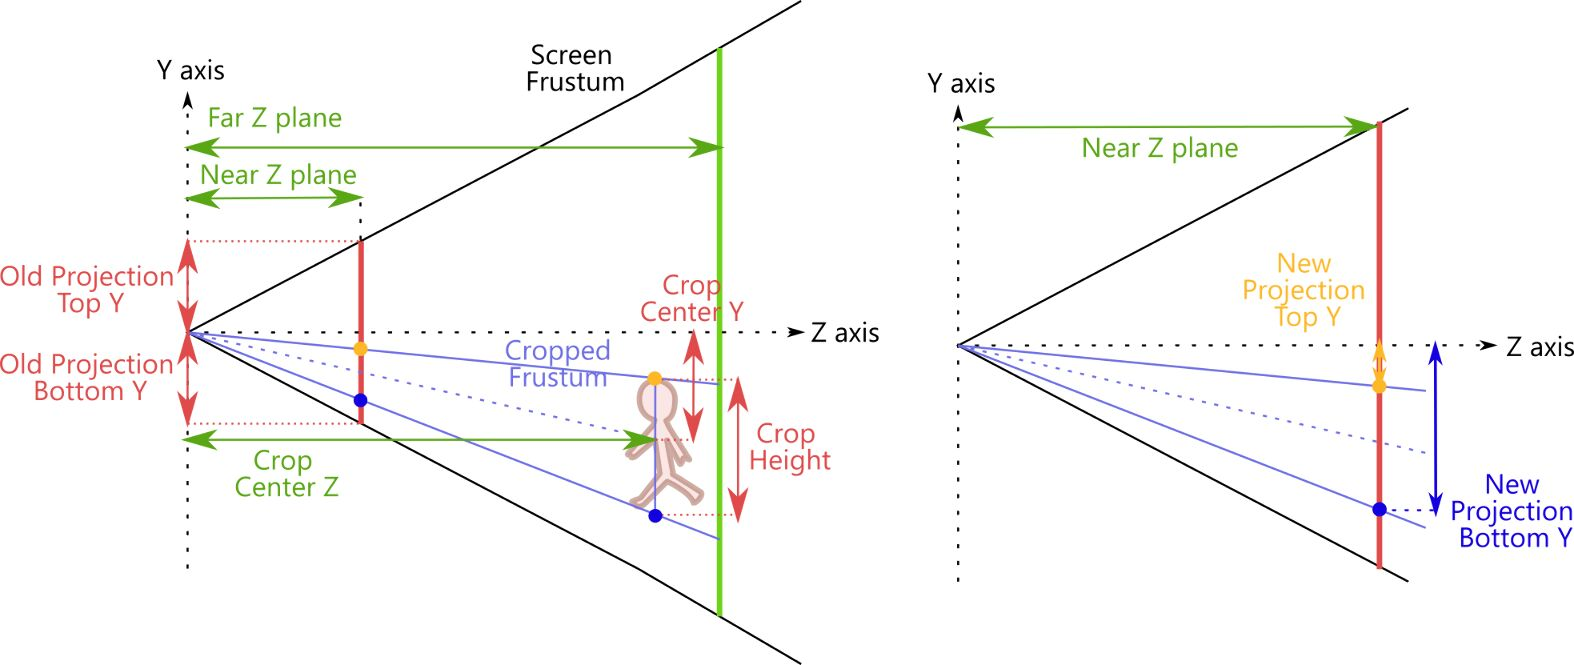
\includegraphics[width=\textwidth]{\imgfp/dynamic_crop/dynamic_crop}
	%\setkeys{Gin}{draft}
	\centering{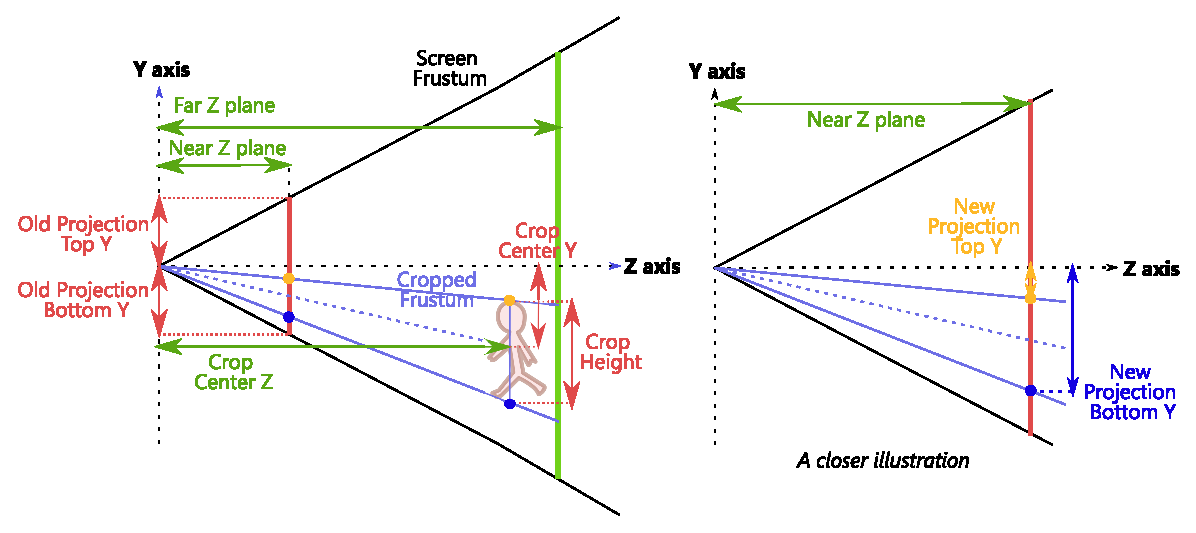
\includegraphics[width=\textwidth]{\imgfp/dynamic_crop/dynamic_crop_vect}}
	%\setkeys{Gin}{draft=false}
	%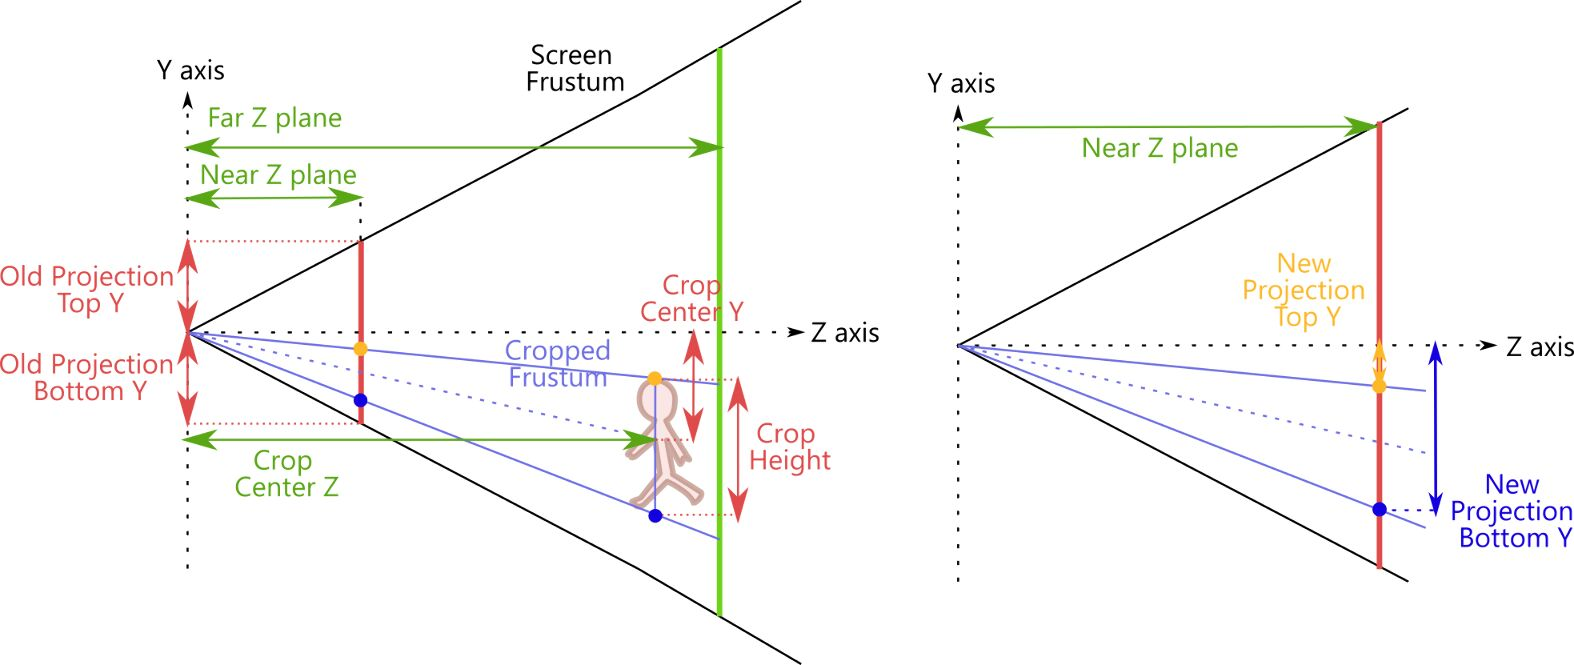
\includepdf[width=\textwidth]{\imgfp/dynamic_crop/dynamic_crop}
	\caption{A 3D space with origin at the camera, and axes aligned with camera directions ($x$ - right, $y$ - top, $z$ - front). The figure shows a slice of this space with $x=0$, illustrating the dynamic projection crop. \textit{(Left)} The near plane of the old screen frustum is defined by a $z$ distance (arbitrary), and $x$/$y$ coordinates of the frustum borders (top/bottom coordinates on illustration). \textit{(Right)} To make the projection cropped around the avatar body, we compute an axis-aligned bounding box of the body, then project its spans onto the near plane, obtaining top/bottom borders, defined by intersection coordinates of the projection lines and the old near plane. The new frustum will have the same near and far planes as the old one, to ensure preservation of perspective.}
	\label{fig:dynamic_crop_math}
\end{figure}
% Since we know This allows us solve Equation \ref{methods:eq:project-zcoord} for 
%\begin{bmatrix} 
%	\tfrac{2n}{r - l} & 0              & \tfrac{r + l}{r - l} & 0 \\
%	0               & \tfrac{2n}{t - b}  & \tfrac{t + b}{t - b} & 0 \\
%	0               & 0                & -\tfrac{f + n}{f - n} & \tfrac{-2fn}{f - n} \\
%	0               & 0                & -1                   & 0
%\end{bmatrix}

Now we need to compute the new cropped frustum parameters: top $t_{new}$, bottom $b_{new}$, right $r_{new}$ and left $l_{new}$ (see Listing \ref{appendix-code:projectioncropper}). We can take $n_{new} = n$ and $f_{new} = f$, since they are unaffected by the cropping operation. We take 3D locations of avatar joints for the given frame, and from minimum and maximum joint coordinates we compute the crop's center $\langle x, y, z\rangle$ and crop extents $\langle H, W \rangle$ in the camera coordinate space. Then, values $\tfrac{H}{z}$ and $\tfrac{W}{z}$ tell how many times the crop area is smaller relative to the original frustum. We can multiply $t$ and $b$ by $\tfrac{H}{z}$; and $l$ and $r$ by $\tfrac{W}{z}$ respectively to shrink the frustum area to the desired size. Now the frustum center needs to be shifted to match the crop in the camera space coordinates. For this we multiply the crop center's coordinates $\langle x, y \rangle$  by $\tfrac{n}{z}$ thus getting projected coordinates of the crop center, and by these coordinates we offset previously scaled $t$, $b$, $l$ and $r$. Again, see how the old and new frustums correspond to each other on Figure \ref{fig:dynamic_crop_math}. Overall, the computation of the cropped frustum looks like:
\begin{align}
	n_{new} &= n & f_{new} &= f \\
	l_{new} &= l\cdot\dfrac{W}{z} - x\cdot \dfrac{n}{z} & r_{new} &= r\cdot\dfrac{W}{z} + x\cdot \dfrac{n}{z} \\
	b_{new} &= b\cdot\dfrac{W}{z} - y\cdot \dfrac{n}{z} & t_{new} &= t\cdot\dfrac{W}{z} + y\cdot \dfrac{n}{z} \label{methods:eq:frustum-new-parameters}
\end{align}

Using Formula \ref{methods:eq:ndc-projection}, we make a new projection matrix from the updated frustum parameters. The matrix can be passed to the previously described GPU shader programs, to render the images. However due to cropping, the inferred avatar image has to be rendered at a specific image location, that corresponds to the initial cropping bounding box in the image space. Since we use a separate rectangle mesh for rendering the inferred images on top, before using the dynamic crop the coordinates of the rectangle corners were:
%\begin{equation}
	\begin{align}
		%\begin{split}
		\text{top{\_}left} &= \langle -1, 1 \rangle & \text{top{\_}right} &= \langle 1, 1 \rangle \\
		\text{bottom{\_}left} &= \langle -1, -1 \rangle & \text{bottom{\_}right} &= \langle 1, -1 \rangle
		%\end{split}
	\end{align}
%\end{equation}

We need to map these coordinates to the cropped frustum's parameters. Since the old frustum's parameters do not necessarily form ranges between -1 and 1, we need to take a corresponding parameter of the cropped frustum and find how it relatively adjusts the old one. For example, a value of relative update by the $r_{new}$ parameter would be $\tfrac{r_{new}}{l - r}$. Thus, the updated image coordinates to render the dynamically cropped image would be:
\begin{align}
	%\begin{split}
	\text{top{\_}left} &= \langle \dfrac{l_{new}}{l - r}, \dfrac{t_{new}}{t - b} \rangle & \text{top{\_}right} &= \langle \dfrac{r_{new}}{l - r}, \dfrac{t_{new}}{t - b} \rangle \\
	\text{bottom{\_}left} &= \langle \dfrac{l_{new}}{l - r}, \dfrac{b_{new}}{t - b} \rangle & \text{bottom{\_}right} &= \langle \dfrac{r_{new}}{l - r}, \dfrac{b_{new}}{t - b} \rangle
	%\end{split}
\end{align}


%	\end{itemize}
%	\item Dynamic camera frustum cropping
%		\begin{itemize}
%			\item Around view span -- On every frame compute coordinates of joints in camera space, find a XY-bounding box for them. Project bounds of this box onto the image, and find adjustments of top-bottom-left-right-near-far parameters of the camera frustum. Calculate a new projection matrix to fit only the bounding box of the avatar. Rasterize an input frame with this matrix. Infer the network and place the output using offset computed from the updated projection matrix
%			\item Auto-zoom to reducing frame waste -- detect if bounding box of joints is cut off by the mobile screen. Zoom in the projection matrix to the avatar to compensate cut off parts. This will allow to see the avatar parts rendered in bigger resolution (thus DNN has to be trained on zoom scale too)

\section{Improving quality of synthesized images}\label{methods:zooms}

%\setlist{  
	%	listparindent=\parindent,
	%	parsep=0pt,
	%}
%listparindent=1.5em, labelsep=2em, itemindent=1.5em, 
% \subsubsection{Hello}

TODO: camera space augmentations explanation
%The baseline DNN architecture \cite{dnn:stylepeople21}, although being state-of-the-art for learning from a few images (or a video sequence) to synthesize full-body (FB) avatars images, may not perfectly suit AR scenario of the mobile application. Previously we proposed to use dynamic projection cropping, to infer the neural renderer and use as much of image resolution as possible. At the very least, this would mean that the computations are spent on useful work, not just background which ought to be segmented out anyway. But also it is to produce more sharp images  to generate avatar's images, since the resolution of the generated images (at least $512 \times 512$ pixels) is already much lower than of the mobile device's screen ($1920 \times 1080$). On the other hand, such dynamic cropping could pass input images of larger scale than FB, for example upper-body or even close-up on a body part such as face. If the neural renderer is not trained to see such zoomed scales, then the produced images will likely be bad. It can be explained by the convolutional nature of this architecture. If convolutional filters are optimized to activate on certain patterns, within their receptive field, then there is no guarantee that the same patterns could be detected from either far-away or a zoomed input image (see Figure \ref{fig:exp:baselines}, where the baseline is trained only on FB inputs, and it cannot generate as good images for the upper-body or close-up face).
%
%Thus, the DNN has to be 

\begin{figure}[ht]
	\centering
	\begin{subfigure}[b]{0.48\textwidth}
		\centering
		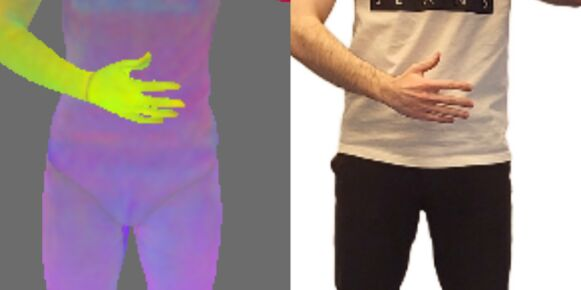
\includegraphics[width=\textwidth]{\imgfp/cam_augs/img}%
		\caption{}
		\label{fig:cam_aug:before}
	\end{subfigure}
	\begin{subfigure}[b]{0.48\textwidth}
		\centering
		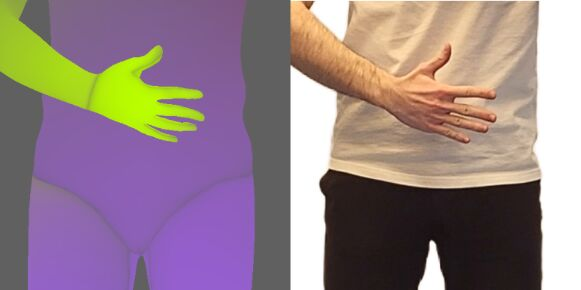
\includegraphics[width=\textwidth]{\imgfp/cam_augs/cam}%
		\caption{}
		\label{fig:cam_aug:after}
	\end{subfigure}
	\caption{(\protect\subref{fig:cam_aug:before}) Implementation of zooming using image-space augmentations. The body mesh is rasterized in full-body, the ground truth is transformed once to be in an alignment with the rasterization. Then both are magnified, loosing a lot of quality. (\protect\subref{fig:cam_aug:after}) Using camera-space augmentations, the virtual camera used for rasterization replicates zooming by moving towards the avatar. The input image can be made arbitrarily sharp. The ground truth image is still transformed with image-space augmentations, but only once, preserving a bit of quality.}
	\label{fig:cam_aug}
\end{figure}

%The baseline DNN architecture \cite{dnn:stylepeople21} proved to be sufficient to render FB images of avatars. However, we found out that the rendering network cannot reliably render parts on the body that were never seen during training, most commonly under boots surface, and top of the head. At best, these places can be rendered as random patches of color, e.g. from clothes or skin. Intuitively it is so, because in these areas the neural texture will contain default values during the whole training process. If the renderer learns quickly enough to map such default values to skin or clothes, the chance is that the texture overall will not move much away from the defaults. Although the unseen parts are not rendered correctly from reconstruction point of view, it does not hurt overall accuracy. On the other hand, there is a chance that the neural texture will significantly move away from the default initialization. Thus, after many epochs the default values contained in the unseen parts will be outliers that the renderer does not expect to see. This may trigger it to render abnormal color or fail segmentation prediction. Attempts on dealing with this artifact will be given shortly after.

Further, we will describe the experiments on DNN training, performed on top of applying camera-space augmentations to train on zoomed images. We will group experiments with similar ideas into paragraphs, which we summarize with a bold emphasis on the font. We also put references to figures that contain such experiments, although the discussion of them is provided in Section \ref{res:training}. We explain the motivation and implementation details where needed. For brevity, we present paragraphs and experiments within them not necessarily in the same order, in which we conducted the research.

\vspace{-15pt}\paragraph{Body joints as augmentation centers}(Fig. \ref{fig:exp:basic-zooms}, \ref{fig:exp:basic-zooms-2})\mbox{}\nopagebreak

Having the Python module for computing camera-space augmentations from the image-space transform, we need to define to which points on the ground truth image we should zoom. Obviously, choosing a random location on the image would not work, as the ground truth frames contain background content. If a point outside the human body is chosen, given that the zooming scale is strong, the person will not be present on the augmented image at all. Consequently, the input rasterization for the DNN will be an empty image. We decided for each frame in the training sequence to use predicted SMPL-X joints locations as augmentation centers. Since they are in 3D, we project them onto the image using a projection matrix that was used for SMPL-X fitting process. Then, we take a subset of the joints, for each we assign a specific zooming scale range and probability of being chosen as an augmentation center. Finally, during training we sample random joints for a batch of images according to the weights, uniformly sample a zoom scale from the corresponding range of scales, and apply the camera-space augmentations to the projected locations of joints. We perform experiments, where we select a subset of major joints: head, feet, palms, pelvis. We experiment with different maximum scale of the zooming range: 2.0, 3.5, 4.5, 8.0. Since only a subset of the joints is used, it is possible that other intermediate body parts may be observed slightly less frequently.

\vspace{-15pt}\paragraph{Body mesh vertices as augmentation centers}(Fig. \ref{fig:exp:zoom-vertices})\mbox{}\nopagebreak

Choosing body joints as augmentation centers is easy to apply. However we suspected, that both the neural renderer and discriminator might overfit to certain body parts appearing more frequently at the certain parts of the screen. At the very least, the joint locations are more biased to be in the center of the frame. We tried to increase the variance in the zooming augmentation, by instead choosing body mesh vertices as augmentation centers. We also wanted to preserve the ability to choose specific weights to certain body parts and their zoom ranges. Thus, we decided to build an association between joints and mesh vertices. We used weights of the joints regressing model from SMPL-X. We noticed, that a certain joint is regressed with the highest weights from the nearby vertices. Hence, we associate a vertex to the joint with the highest regressing weight (see Figure \ref{fig:smplx-vert2joint} with examples for a few joints).  We also need for each ground truth image to find 2D projections of all the vertices, similarly to the joints projections. Then, to compute camera-space augmentations we would randomly sample a joint, then uniformly sample a random vertex attached to the joint, and uniformly sample a scale of zooming associated to the joint. 

We perform experiments with the same distribution of joints and zoom ranges as in the experiments above. We also experiment with making a fair distribution of zooming to all body parts. Note that taking the same weights of joints will not accomplish that. This is because the SMPL-X body mesh has different density of vertices, there are about as many vertices in the head as in the other body parts combined. Thus, we  tried to take all vertices associated with a joint, find their extents along $x$, $y$ and $z$ axes, and compute a volume of this bounding box. Then by taking a ratio of the number of joint-associated vertices to the volume, we find the density of vertices around a single joint. For camera-space augmentations, we try to take joints weights, that would equalize this density. Thus we hope to achieve the uniform distribution of body parts images during training.

\begin{figure}[!htpb]
	\centering
	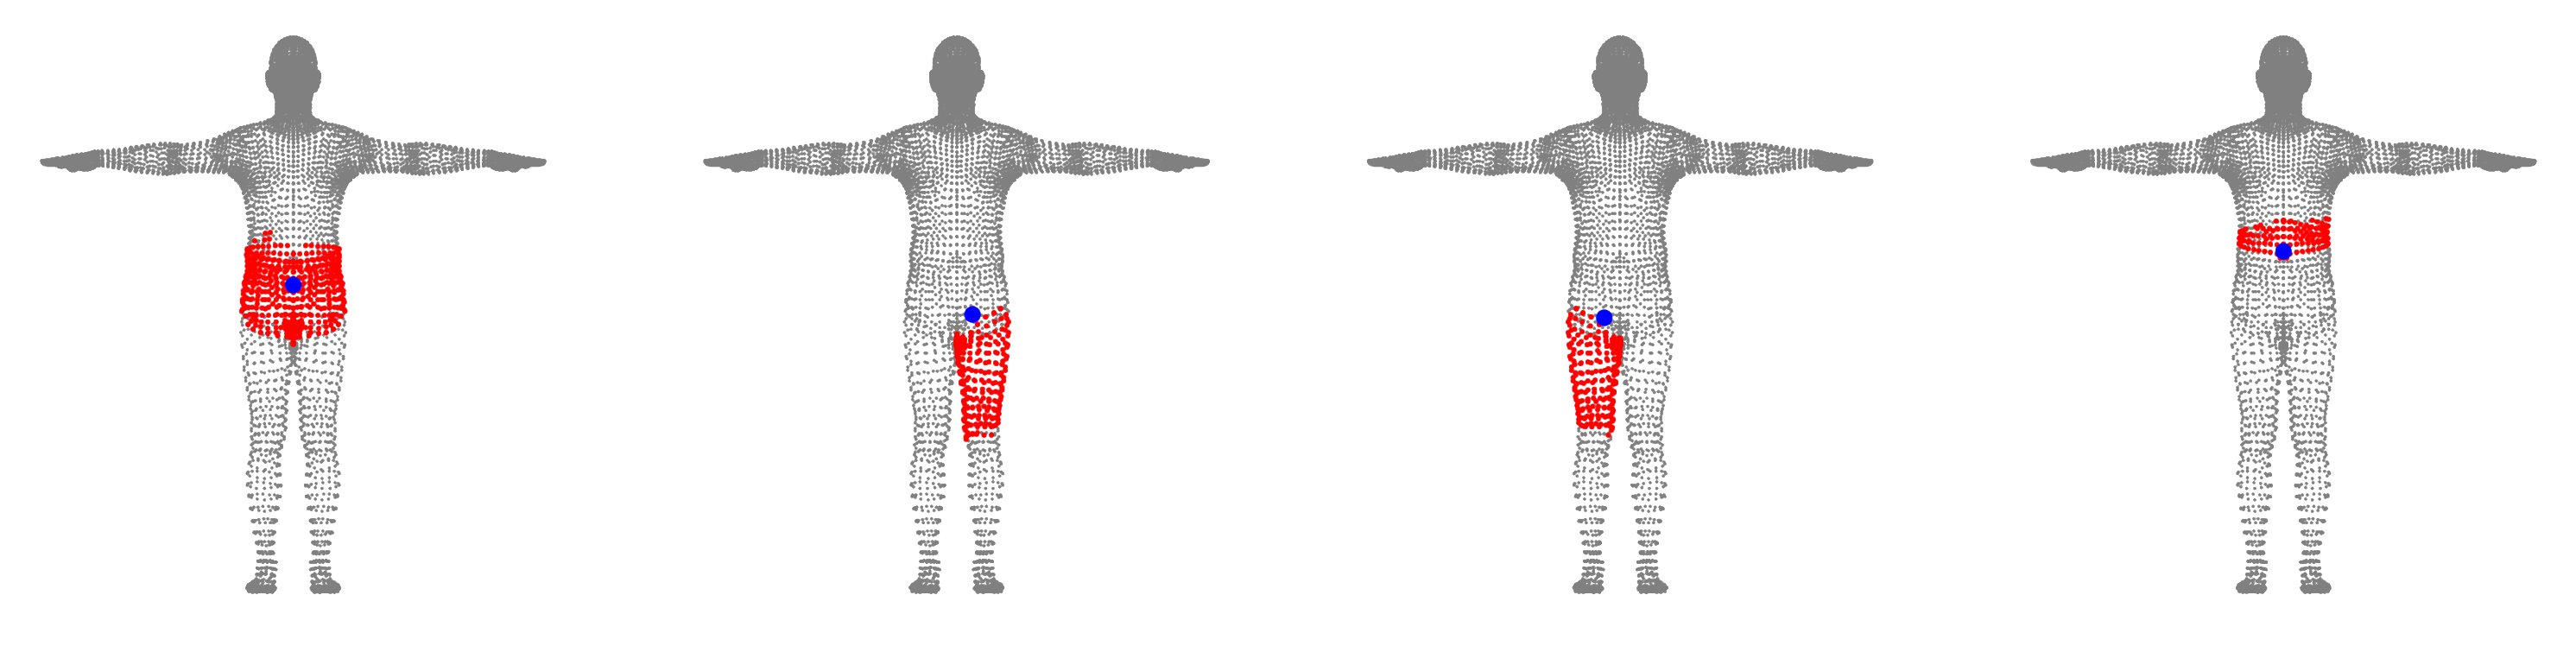
\includegraphics[width=\textwidth]{\imgfp/smplx/one-joint-vertices}%
	\caption{Assignment of mesh vertices (red) to body joints (blue). For each vertex, we take the joint with the most significant skinning weight from SMPL-X body model, that determines how movement of the joint affects the given vertex's movement. We use this assignment to select mesh vertices as centers of camera-space augmentations. We speculate that choosing vertices rather than plain joints improves augmentations variance and decreases overfitting.}
	\label{fig:smplx-vert2joint}
\end{figure}

\vspace{-15pt}\paragraph{Increased learning rate for the neural texture}(Fig. \ref{fig:exp:ntex-lr-higher})\mbox{}\nopagebreak

During experiments with zooming, we observed that gradient tensors of the neural texture have norm values that are typically an order of magnitude lower than of the neural renderer or discriminator. We experimented with increasing the learning rate of the neural texture by either 5 or 10, to compare the outcomes.

\vspace{-15pt}\paragraph{Train with zoomed scale and fine-tune with FB scale only}(Fig. \ref{fig:exp:fine-tune-wo-zooms}, \ref{fig:exp:fine-tune-wo-zooms-texlowerlr})\mbox{}\nopagebreak

From the above experiments we noted, that by training on zoomed images, although we indeed achieve more realistic results on zooms, the quality of FB images decreases, compared to the baseline. On one hand it is logical, because the neural renderer is much less frequently tasked with rendering FB scale images. On the other hand, by training on FB scale only, the ground truth images in resolution $512 \times 512$ lack a lot of fine-grained details, partically due to bilinear interpolation in the augmentations. We expected that by seeing zoomed images, the neural renderer and the neural texture will learn more of such details from the ground truth images, possibly improving the FB scale as well. However, we did not observe FB improvement. We then tried to train the architecture on zoomed images with further fine-tuning for FB images.

%Furthermore, the learning capacity of the neural renderer might be dispersed to learn to draw the whole range of scales, thus under-performing on FB. 
We tried to decrease learning rate for the neural renderer and the neural texture by some factor. We try the following combinations of factors (the 1\textsuperscript{st} for the neural renderer, the 2\textsuperscript{nd} for the neural texture): $(1, 1)$, $(0.5, 1)$, $(0.2, 1)$, $(0.1, 1)$, $(0.5, 1)$, $(0.5, 0.5)$, $(0.2, 0.5)$, $(0.1, 0.5)$.

\vspace{-15pt}\paragraph{Collecting BN statistics only on either FB or zoomed scale}(Fig. \ref{fig:exp:bnf-statfb-statzooms}, \ref{fig:exp:scale-distr-enable-disable-stat-or-gan}, \ref{fig:exp:a03-uniform}, \ref{fig:exp:bnf-disable-track})\mbox{}\nopagebreak

We had a suspicion, that BN layers inside the architecture may behave wrong, when normalizing batches of data with different scales of zooms. For example, when the neural renderer or discriminator processes a frame with a close-up on either face or foot, the statistics of the batch may have high variance, and averaging them may result in gradual instability of the training. On the other hand, FB images are more consistent, they always show both the head and feet in the similar proportions. Thus, we separately pass batches of FB scale and zoomed scale images. We use batches of FB 20\% of times, and batches of zoomed frames 80\% of times. We experiment with disabling BN layers across the whole architecture, either only for zoomed batches, or conversely only for FB batches (as a wild hypothesis). 

Note that in PyTorch terms, disabling of BN means that the affine parameters will not be optimized, and the running average statistics will not be updated, and they will be used for normalization of the data. Additionally, we experiment with using batch statistics instead of running average statistics to normalize the data when BN layers are disabled. We also try passing zoomed images much more rarely, as well as combining it with zooming to body mesh vertices uniformly. 

\vspace{-15pt}\paragraph{Alternative normalization layers instead of BN}(Fig. \ref{fig:exp:different-norms})\mbox{}\nopagebreak

We continued to analyze the aforementioned discrepancy of batch statistics when training on zoomed scale. We try to replace the BN layers with other normalization layers across the whole architecture. We try Instance Normalization layers \cite{dnn:in16}, Group Normalization layers \cite{dnn:groupnorm18}, as well as removing all the BN layers. Since we train both the neural renderer and discriminator from scratch, there are no architectural issues with replacing BN layers inside the well known architectures that are used in the baseline (ResNet18, StyleGAN's discriminator).

\vspace{-15pt}\paragraph{Instance Normalization layers instead of BN}(Fig. \ref{fig:exp:instancenorm-other-seq}, \ref{fig:exp:instancenorm-and-switch-track-stat})\mbox{}\nopagebreak

After noticing, that Instance Normalization layers both perform better and can be launched on our mobile hardware, we check that the visual quality is admissible when using other training sequences. Since in PyTorch by default Instance Normalization layers do not collect running instance statistics (as BN layers do) that are used for inference, we also try to enable this behavior.

\vspace{-15pt}\paragraph{Removing BN layers from parts of the architecture}(Fig. \ref{fig:exp:nonorm:r:rd:r+dinstancenorm}, \ref{fig:exp:nonorm:d:rd:rhead})\mbox{}\nopagebreak

In pursue of finding which BN layers in the architecture are prone to fail more, we try to partially remove BN layers: from the neural renderer; from the last layers of the neural renderer; from the discriminator; from both the neural renderer and discriminator; from the neural renderer, and replacing discriminator BN layers with Instance Normalization layers. By doing so, we expect that the visual quality could improve for some experiments, which would imply the correctness of our hypothesis on batch statistics of zoomed images. If otherwise the quality decreases, then the issues might be anywhere else, or prove that normalization layers of any kind are crucial for convergence, even at a cost of visual artifacts or overfitting.

\vspace{-15pt}\paragraph{Using BN layers without learned affine parameters}(Fig. \ref{fig:exp:norm-noaffine}, \ref{fig:exp:bnf-disc-noaffinenorms}, \ref{fig:exp:renderer-noaffinenorm})\mbox{}\nopagebreak

Apart from the running average statistics, there are also learned affine parameters in the Batch and Instance Normalization layers ($\gamma$, $\beta$ as in Formula \ref{lit:eq:bn}), which also may fail to converge properly because of the zoomed scale images. We thus try to make these parameters constant $\gamma=1$, $\beta=0$. We experiment with applying it:
\begin{itemize}
	\item in the neural renderer;
	\item in both the neural renderer and discriminator;
	\item with normalization statistics collected only on FB frames, and without affine parameters in the discriminator (or discriminator with all Instance Normalization layers);
	\item with normalization statistics collected only on FB frames, and without affine parameters in the discriminator or both neural renderer and discriminator;
	\item  with normalization statistics collected only on FB frames, all BN layers replaced with Instance Normalization layers, and without affine parameters in both neural renderer and discriminator;
\end{itemize}

\vspace{-15pt}\paragraph{Modifying optimization of neural texture's unused parameters}(Fig. \ref{fig:exp:nza-or-bnfix}, \ref{fig:exp:nza-bnfix-zoomvertices}, \ref{fig:exp:nza-bnfix-finetune}, \ref{fig:exp:nza-bnfix-ntex8})\mbox{}\nopagebreak

Adam \cite{dnn:adam14} optimizer that is used for all learnable parameters in the baseline architecture, stores momentum of all the parameters' gradients in a form of exponential average. In theory, this helps to get stability of optimization when encountering abnormal or invalid training data. Making an optimization step with a gradient, which was resulted from such data may be harmful. The momentum prevents too abrupt adjustments to the previous direction of optimization. 

When we rasterize input frames with a neural texture, only at most half of the texture's pixels will be present. For example, when rasterizing a frontal view of a person, all the pixels for the back view will be absent. Thus, only the seen portion of the pixels will receive a non-zero gradient value. Although all the other pixels will not update on the current step, their momentum will decay in Adam optimizer. We hypothesize, that we can improve the training, by changing the Adam's algorithm to prevent decaying of momentum for parameters that received no gradient on an optimization step. Our motivation, is that the momentum direction that is currently stored for the unseen pixels of the neural texture will still be fairly correct even after updating the seen pixels, because they store very independent information.

We apply this adjustment by reusing Adam algorithm implementation from PyTorch, and by using masked operations when decaying the momentum tensors. The mask filters out parameter positions, where the computed gradient values are near zero. We train with this modified optimizer and compare it with a normal train on zoomed images (to the joints). We then add other adjustments, such as collection of BN layers statistics only on FB scaled frames and then:
\begin{itemize}
	\item choosing body mesh vertices as centers of augmentations;
	\item fine-tuning on FB scaled frames;
	\item trying a batch size equal to 1, so that batch statistics will effectively be instance statistics, possibly proving that discrepancy of batch statistics may cause the visual artifacts (see the experiment's results on Figure \ref{fig:exp:batch-size-1}).
\end{itemize}

\vspace{-15pt}\paragraph{Disabling GAN losses on zoomed scale}(Fig. \ref{fig:exp:scale-distr-enable-disable-stat-or-gan}, \ref{fig:exp:bn-momentum-high})\mbox{}\nopagebreak

The learning from competition, which is what the GAN approach in essence is, may be both advantageous and harmful. This may apply to the zoom scaled images as well. If the discriminator network is too accurate in distinguishing the real zoomed images from synthesized ones, then the generator may never succeed fooling it. This example of a "lost" competition may drastically decrease the final quality of the neural renderer. We thus experiment with taking the experiment where BN layers are disabled for zoomed images, and disable execution and optimization of the discriminator only for zoom scaled batches; or only for FB scale batches (as a wild guess). This also means removing the Adversarial and Feature-Matching losses from optimization. We also conduct another experiment with removing these losses for the whole training.

\vspace{-15pt}\paragraph{Collecting BN statistics with high momentum, only on FB scale}(Fig. \ref{fig:exp:bn-momentum-high})\mbox{}\nopagebreak

Another source of possibly corrupted running average statistics of Batch Normalization layers may be in the rate of exponential decay with which they are collected (also referred to as momentum). By default, the BN layers have a decay rate 0.1, meaning that statistics of a single batch may still be significantly present in the running average of up to 30 next batches (e.g. $(1-0.1)^{30} \approx 0.04 = 4\%$ of the values still present after 30 batches). We experiment with a higher decay rate: 0.2 (significant for $\approx 15$ batches), 0.3 (significant for $\approx 9$ batches).

\vspace{-15pt}\paragraph{Processing multiple batches before making an optimization step}(Fig. \ref{fig:exp:optimizer-step-n})\mbox{}\nopagebreak

A fairly small batch size (8) may also cause instability of statistical properties within a batch. We cannot try a higher batch size because of a memory limit on the hardware during training. However, we experiment with simply performing an optimization step every $k$ batches instead of every single batch. Although it is not equivalent to the higher batch size, because the BN statistics are anyway averaged and added after processing every batch, the affine parameters are optimized using an average gradient, which may include information from a wide range of zoomed scales and body parts. The same applies to updating of all the learned parameters in the architecture, including the neural texture, convolutional layers of the neural renderer and discriminator. We try making the optimization step every 2 or 4 batches, as well as updating only discriminator every 2 batches (a technique proposed for improving GAN performance in \cite{dnn:gan14}).

\vspace{-15pt}\paragraph{Collecting BN statistics only on FB scale, fine-tuning only on FB scale}(Fig. \ref{fig:exp:bnf-fine-tune}, \ref{fig:exp:filter-shade-fine-tune})\mbox{}\nopagebreak

We combine the experiments on collection of statistics of BN layers only on full-body scaled images, and fine-tuning it after a certain epoch to only FB scale. Thus, during fine-tuning the statistics are collected from all the training data. We also try lower the learning rate of the neural texture, either decreased by 10 times, or by 1000 times. It has a motivation of preventing drastic updates of the neural texture, after is captured fine-grained details from the zoomed scales. The fine-tuning should restore the original FB quality, and possibly suppress the artifacts resulted from the zoomed training.

\vspace{-15pt}\paragraph{Non-uniform distribution of augmentation zoom scales}(Fig. \ref{fig:exp:a03-bl})\mbox{}\nopagebreak

Previously, we applied the camera-space augmentations by uniformly sampling a random zooming scale within a specified range. We later hypothesize, that it may be undesireable, as the FB frames will be less likely to be shown, e.g. for a range of scales between 0.7 and 3.5 (which is a moderately high zoom), the FB range is only within 0.7-1.1 scales, which is only 15\% of the whole range. Hence, it is pointless to expect high quality of FB images. Moreover, we had a quick debugging experiment on learning with ever so rarely shown zoomed frames, and it hinted that adequate zoomed images can be learned, even if they are shown rarely. In this group of experiments, instead of a single range of scales with a uniform sampling, we use multiple bands of ranges, each having a weight. By changing the weights and ranges size, we can make some range of zooming scales more probable than the others. We use it to train on mostly FB images, with a gradually decreasing probability of higher zoom scales, up to $\times12$ scale.

\vspace{-15pt}\paragraph{Using the same scale of zoom augmentations within a batch}(Fig. \ref{fig:exp:bnf-samescalebatch-nomultiscaletex-highdice})\mbox{}\nopagebreak

Following the hypothesis of incompatible statistics of zoomed frames, which may cause instability of training with BN layers, we try to restrict every training batch to have the same scale of zooming, the same affine rotation rotation and the same center of camera-space augmentations, thus making the zoomed frames statistics as much comparable as possible.

\vspace{-15pt}\paragraph{Disabling Adam optimizer's first momentum}(Fig. \ref{fig:exp:optimizer-momentum})\mbox{}\nopagebreak

After experimenting with collection of statistics for the BN layers from FB scaled images, we suspected that the Adam optimizer's momentum may occasionally push the optimization towards a certain harmful direction for many batches, due a slow decay of the running exponential averaging (0.9 by default). We experiment to check this suspicion, by setting the first momentum to 0.0, for the neural texture, or for the neural texture plus the discriminator.

\vspace{-15pt}\paragraph{Strong affine augmentations}(Fig. \ref{fig:exp:strong-affine-aug})\mbox{}\nopagebreak

As a regularization technique, we experiment with increasing the variance of affine augmentations. We apply a very strong translation (so that sometimes the avatar body parts may be just barely in the input frame), and very strong rotation (used to be $\pm 45^\circ$, and we try $\pm 90^\circ$). This should reduce both overfitting and discrepancy when rendering body parts at different screen locations, e.g. the image's middle, borders, corners. The rotation additionally can improve inference quality on mobile, as in AR it's possible to rotate the mobile device and thus observe the avatar horizontally or even upside down, for which the neural renderer is unlikely to be trained.

\vspace{-15pt}\paragraph{Gradient clipping}(Fig. \ref{fig:exp:gradclip-constant-or-mean}, \ref{fig:exp:gradclip-mean-fraction}, \ref{fig:exp:gradclip-scheduler})\mbox{}\nopagebreak

The next regularization approach we use is gradient clipping, that should reduce optimization steps from gradient tensors that have too high norm values, and if such steps were made, it could lead us to an unpredictable location on the optimization landscape. Thus the gradient tensors with an exceeding norm value are normalized to a certain limit. It may also help to prevent overfitting towards training samples which are outlying or invalid, since they are a minority among the training samples, the clipped optimization steps are unlikely to hurt the training process.

We try to clip gradients of both the neural renderer and discriminator to norm 5.0, or to 2.0. Alternatively, we find a mean norm independently for the neural renderer and discriminator, and use it multiplied by either 1.0, 0.5 or 0.2 as a gradient clipping limit. It should effectively act as a lower learning rate, since the majority of gradients will be clipped. However, we also expect appearing of much fewer overfitting artifacts. We also experiment with adding a decaying learning rate scheduler, with a warmup period that sets up to $10^{-2}$ learning rate to the neural renderer, and gradually decays to learning rate $10^{-6}$. We add the gradient clipping with an intuition, that it will help to preserve stability of optimization during the warmup with too high learning rate.

\vspace{-15pt}\paragraph{Weight decay}(Fig. \ref{fig:exp:wdecay-nr2:nronly}, \ref{fig:exp:wdecay-nr2:ntex1+disc}, \ref{fig:exp:wdecay-nr2:ntex2+disc}, \ref{fig:exp:wdecay-nr3:ntex+disc}, \ref{fig:exp:wdecay-nr432}, \ref{fig:exp:wdecay-nr654})\mbox{}\nopagebreak

Another regularization approach that we explore is weight decay (also referred to as L1 regularization) on the learned parameters across the whole architecture. It should prevent overfitting by slowly pushing the weights tensors towards zero L1 norm. Thus, it decreases a chance of learning very high-magnitude weights, which is a common symptom of overfitting and instability of outputs. There is a known issue with Adam optimizer that it does not implement the weight decay in a mathematically correct way, thus we use AdamW \cite{aux:adamw17} modification that solves it. We experiment with weight decay of neural renderer's parameters to norm values $\{10^{-i}\}^{6}_{i=0}$. Together with the found promising weight decay value of $10^{-2}$ for the neural renderer, we experiment with weight decay of the neural texture and discriminator with the following values: $(10^{-1}, 10^{-1})$, $(10^{-1}, 10^{-2})$, $(10^{-2}, 10^{-1})$, $(10^{-2}, 10^{-2})$. We also try weight decay $10^{-3}$ value for neural renderer alone; for neural renderer plus discriminator; and for neural renderer, discriminator and neural texture together.
%\lipsum[1-1]

\vspace{-15pt}\paragraph{Dropout for channels of activation tensors}(Fig. \ref{fig:exp:dropout-e-d}, \ref{fig:exp:dropout-ed-ed}, \ref{fig:exp:dropout-all-conv-ed-ed})\mbox{}\nopagebreak

We try to add regularization to the neural renderer via 2D dropout layers \cite{aux:dropout2d-15} to randomly zero-out (completely) a few random channels of activation tensors. We experiment with adding dropout with probability $p \in \{0.1, 0.05\}$ after all levels of either encoder or decoder or them both. We also try to apply it after every single convolution in the neural renderer, with $p \in \{0.1, 0.15, 0.2\}$. In theory this should force learning of multiple slightly similar convolutional filters that would act as backup to fit the training images in a presence of dropout, and then to provide stability of outputs during inference.

\vspace{-15pt}\paragraph{Additive noise to neural texture's initialization}(Fig. \ref{fig:exp:add-noise-ntex-init})\mbox{}\nopagebreak

The neural texture's initialization with spectral mesh coordinates (see Figure \ref{fig:spectral_ntex}) may contain values with a large magnitude. We hypothesize, that it may be an issue for body parts may be never shown on the ground truth images (bottom of shoes, armpits, top of the head). The texture pixels that correspond to those parts will never be changed away from the default initialization. Thus, after optimization, the contained values may be well beyond a typical range of values, causing the neural renderer to produce unstable results. We experiment with adding a random Gaussian noise (with $\sigma\in\{0.1, 0.025\}$) to the texture intialization, with an idea to partially randomize the unseen body parts on the texture, and reduce the appearing artifacts (see also Figure \ref{fig:ntex-grad-artifact-fixed}). We also try a random neural texture intialization, to understand how convergence of the neural renderer depends on the baseline initiliazation, and whether the similar artifacts emerge.

\vspace{-15pt}\paragraph{Additive noise augmentation for input and ground truth data}(Fig. \ref{fig:exp:add-noise-input}, \ref{fig:exp:add-noise-ntex}, \ref{fig:exp:add-noise-rgb})\mbox{}\nopagebreak

We try to regularize the neural renderer by applying a random additive Gaussian noise to the input frames (with $\sigma\in\{0.01, 0.02, 0.1\}$), i.e. affecting appearance of both the background and the body mesh on a frame. Alternatively, we add it to the neural texture before input frame rasterization (with $\sigma\in\{0.01, 0.02, 0.1\}$), i.e. affecting only the body mesh. Lastly, we try adding it to the ground truth images (with $\sigma\in\{0.05, 0.1\}$). This might make the network overfit less to subtle misalignment of body mesh fits, and instead encourages to save similar information in multiple parameters of the neural texture or the neural renderer.

\vspace{-15pt}\paragraph{Reducing the number of parameters in the neural renderer}(Fig. \ref{fig:exp:neural-renderer-capacity})\mbox{}\nopagebreak

It is a common practice in the encoder-decoder based DNN models to have a much bigger number of learned parameters in the encoder rather than in the decoder \cite{dnn:resnet-unet20, dnn:relightable-pointcloud20, dnn:neuralpointgraphics20}. This is because the encoder's task of data compression into a smaller decodable size is harder than decompressing it. Still, we experiment with reducing the number of learned parameters in the encoder, by discarding the last convolution of the last level of ResNet18, effectively reducing the number of parameters in the neural renderer by 20\%. We also try to reduce the number of output channels for all decoder levels by half, reducing the number of neural renderer parameters by 25\%. This may act as regularization, that prevents overfitting.

\vspace{-15pt}\paragraph{Reducing the number of parameters in the neural texture}(Fig. \ref{fig:exp:nza-or-ntex8}, \ref{fig:exp:bnf-samescalebatch-nomultiscaletex-highdice})\mbox{}\nopagebreak

The default neural texture has multiple downscales learned jointly with the neural texture in the original resolution. We referred to it as a multi-scale neural texture. We experiment on collecting statistics of BN layers only from FB scaled images, but also training without those downscales of the neural texture (i.e. only $512 \times 512$ pixels resolution). Perhaps, the lowest resolution downscales of the texture may learn values, that when upsampled and added to the original resolution may change the values in the pixels, that correspond to the body parts that may not be seen on the ground truth images. This can cause values on the rasterized input frames that are abnormal for the trained neural renderer, and thus the visual artifacts with failed segmentation that we encountered.

We also try to take a standard experiment with zooming to joints, and then reducing the number of neural texture channels from 16 to 8. With that we try to understand importance of pixel-wise depth of the encoding for different body parts, and how it affects the visual quality.

\vspace{-15pt}\paragraph{Pass downsampled input to levels of the neural renderer's encoder}(Fig. \ref{fig:exp:pass-input-in-encoder})\mbox{}\nopagebreak

There are a few successful attempts in the literature \cite{dnn:relightable-pointcloud20, dnn:neuralpointgraphics20} for the generative models with an encoder-decoder architecture, to pass downsampled input frame to the levels of the encoder. This may reduce an effect of data propagation through the model with irreversible accumulation of errors. By reminding the encoder levels how the input data looks like, it may improve compression of the input into the values of bottleneck activations. Thus the learning process may be more stable. We experiment with replacing a few channels of intermediate activations with the downsampled input, which preserves the performance of inference (for possible execution on mobile devices). Alternatively, we try concatenation with intermediate activations instead, and thus having more learnable parameters.

%\lipsum[1-1]

\vspace{-15pt}\paragraph{Adjust weights of training losses}(Fig. \ref{fig:exp:loss-weights}, \ref{fig:exp:bnf-samescalebatch-nomultiscaletex-highdice})\mbox{}\nopagebreak

The baseline architecture uses specific weights for training losses. Namely, Adversarial and Feature-Matching losses contribute with about 25 times lower weight. We try to set all the weights to 1, with motivation that the architecture will start satisfying all the losses, without the need for hyperparameter tuning to different training sequences. Although the magnitude of different losses may be incomparable, we believe, that ever since the Batch Normalization is used in most of DNN architectures nowadays, the specifically chosen loss weights matter less and less. 

We also try to improve the segmentation artifact appearing in the experiments where BN statistics are collected from FB scaled frames. We try to double the segmentation (Dice) loss and compare the effect.

\vspace{-15pt}\paragraph{Use fewer training samples}(Fig. \ref{fig:exp:27-frames}, \ref{fig:exp:filter-shade-fine-tune})\mbox{}\nopagebreak

In the previous experiments we frequently encounter overfitting due to training on zoomed scaled images. We experiment, how the number of training samples affects the training. With too many samples there is a chance that the architecture will generalize well to all of them. On the other hand it may fit well all of them except for a few, that are too complex or invalid (having bad segmentation or SMPL-X fit in the dataset). Thus, these frames will be dominant in the magnitude of the losses, forcing the architecture to overfit to them no matter what, thus the artifacts (see Figure \ref{fig:overfitting_rotation}). We try to reduce the number of training samples from 397 to 27, that were manually selected to show the person from all the sides, and most of the adequately fit poses. We also try use the original training sequence, but manually removing a handful of frames that are fit badly by the neural renderer in most of our experiments (e.g. the ones containing change of lighting such as on Figure \ref{fig:overfitting_gt} to the left).

\vspace{-15pt}\paragraph{Learned MIP-maps of the neural texture}(Fig. \ref{fig:exp:ntex-mip-maps})\mbox{}\nopagebreak

In the baseline architecture the library Nvdiffrast \cite{aux:nvdiffrast20} for differentiable rasterization allows applying MIP-maps (see Figure \ref{fig:mipmap}) to the neural texture. However, the algorithm they use to generate the downscaled levels of the texture does not include any filtering, instead it only averages 4 neighboring pixels. The library allows to pass custom tensors as the MIP-maps, thus we try to make these tensors as learned parameters. Our motivation is that in those MIP-maps may be learned information for adjusting the rendering with respect to scale of zoom, since the far-away and full-body scales will be rendered with low-resolution MIP-maps, while the zoomed frames with high-resolution MIP-maps plus the main texture. We initialize the MIP-map tensors with a downscaled version of neural texture's initialization. We do not synchronize the values learned in the neural texture and its MIP maps anyhow. To check the effect of the default MIP-mapping algorithm, we try disabling usage of any MIP-maps whatsoever.
%\lipsum[1-1]

%Researched adjustments:
%\begin{itemize}
%	\item Camera space affine augmentations module (for Python) to eliminate need of augmenting prerasterized frame (which will lead to quality loss on strong zooms)
%	\item Zooming to different joints (or mesh vertices) with different scale range 
%	\item Regularization of Batch Normalization layers to prevent overfit (and Spurious Correlations as result): collecting statistics on FB scale only, or on zoom scale only; using current statistics to train or not
%	\item Accumulating gradients for more than 1 batch before making optimization step
%	\item Adam Optimizer without 1st momentum in neural renderer, discriminator
%	\item Fine tuning a zoom-trained model on FB to restore FB quality and to preserve neural texture high frequency details
%	\item Other normalization layers: Instance norms, Group norms, No norms
%	\item Adam optimizer of the neural texture - do not decay momentum of pixels with 0 analytic gradient (unseen in the current batch)
%	\item Capacity of neural texture, encoder, decoder
%	\item Gradient norm clipping
%	\item Learning rate scheduling with warmup and later annealing
%	\item Concatenate input neural image to deeper activations of the encoder
%	\item More strong affine augmentations 
%	\item Batch normalization without learned affine parameters, or without tracking running statistics 
%	\item Single-scale neural texture, compared to multiscale-texture
%	\item Homogeneous augmentations in a single optimization batch (to prevent mixing of statistics)
%	\item Disabling GAN losses
%	\item Initializing neural texture training from a stable pretrained checkpoint, or random noize, compared to spectral initialization
%	\item Disable discriminator on zooms, or disable discriminator on FB
%	\item Equal loss weights
%	\item Using scale probability distribution to prioritize FB scale and show close-up and far-out ever so rarely
%	\item Dropout2d to nullify random feature maps after convolutions: in encoder, in decoder, in both
%	\item Change input rasterization background to not 0 (which is a valid value on the neural texture), but to ntex.abs()*2
%	\item Add gaussian noize to input rasterization, or neural texture, or ground truth
%	
%\end{itemize}